\section{Problem statement} \label{problem}
\subsection{Notation and definitions}

A \emph{robot} is a kinematic chain the configuration of which is
denoted by \mbox{$q \in \mathcal{C}$}, where $\mathcal{C}$ is the
robot configuration space.

The robot position is represented by the $x$, $y$ components
and yaw rotation $r_z$ of a reference body in the 3D space and is
denoted \mbox{$\mathbf{x} \in \text{SE}(2)$, $\text{SE}(2)$} the rigid
motions in the 2D space.  The height $z$, roll $r_x$ and pitch $r_y$
of the reference body are stored with the kinematic chain angles.

This reference body is often the body attached to the root of the
kinematic chain. In this paper, the position of the robot waist
defines the robot position. Therefore the robot configuration is:

\begin{equation} \label{eq:cfg}
  \begin{aligned}
    \mathbf{x} &= [x, y, r_z]\\
    \mathbf{q} &= (\mathbf{x}, [z, r_x, r_y, \mathbf{q}_{\text{int}}])
    \in \mathcal{C} = \text{SE}(2) \times \mathcal{C}_{\text{int}}
  \end{aligned}
\end{equation}



Therefore a \emph{trajectory} is a continuous function $\gamma$
associating to each point of time of the interval
\mbox{$[t_{\text{min}}, t_{\text{max}}]$} a particular robot
configuration \mbox{$\textbf{q}(t)$}:

\begin{equation} \label{eq:traj}
  \begin{aligned}
    \gamma \colon [t_{\text{min}}, t_{\text{max}}] &\to \mathcal{C}\\
    t &\mapsto \mathbf{q}(t)
  \end{aligned}
\end{equation}


A \emph{rigid transformation} is

\begin{equation} \label{eq:rigidtrans}
  \begin{aligned}
    m \colon \text{SE}(2) \times \mathcal{C}_{\text{int}} &\to \text{SE}(2) \times \mathcal{C}_{\text{int}}\\
    (x, \mathbf{q}_{\text{int}}) &\mapsto (m . x, \mathbf{q}_{\text{int}})
  \end{aligned}
\end{equation}


Walking is a sequence of one or many \emph{footstep(s)}. At the
beginning, both feet are on the floor. This phase is called
\emph{double support phase}. Then, a foot moves until it reaches a
desired position. This interval of time, until the foot lies on the
floor again is called a \emph{single support phase}. The moving foot
is the \emph{swing foot}, the static foot is the \emph{support foot}.

A footstep position is a 2D position on the plane. Steps will be
denoted by \mbox{$S \in \text{SE}(2)$}.

A walking movement can be described as a sequence of footsteps $S_i$,
\mbox{$0 \leq i \leq n^{\text{step}}$}. Step duration is constant and equal
to $T_{\text{step}}$.


\subsection{Trajectory following: from mobile robots to humanoids}


As trajectory following has been extensively studied, a direct use of
previously studied ideas such as illustrated by Fig.~\ref{fig:system}
would seem natural. However, this section will demonstrate that this
naive approach is not sufficient.


Fig.~\ref{fig:system} depicts what would be a mobile-robot closed loop
tracking system applied to a humanoid robot. The reference trajectory
$\gamma$ would be modified by a feedback provided by some external
localization system integrated to the robot and providing an
estimation of the robot position and orientation denoted by
$\hat{\mathbf{x}}$. From this estimation, an error is computed and
added to the original trajectory component by component using a
proportional gain, i.e.\ $k_x$, $k_y$, $k_{r_z}$ on the figure.


\begin{figure}[ht!]
  \begin{center}
    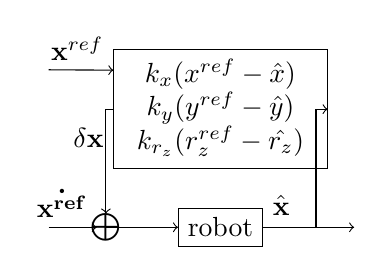
\begin{tikzpicture}[x=.40\textwidth,y=2.5cm]

      \path node (plus) at (-0.45,0) [shape=rectangle,draw,color=white]
            {\color{black} $\bigoplus$};

      \path node (robot) at (-0.15,0)
            [shape=rectangle,draw,label=3:$\hat{\mathbf{x}}$] {robot};

      \path node (errorcomp) at (-0.15,0.6)
            [shape=rectangle,draw,label=185:$\mathbf{\delta \mathbf{x}}$]
            {$\begin{array}{c} 
                k_x (x^{ref} - \hat{x})\\
                k_y (y^{ref} - \hat{y})\\
                k_{r_z} (r_z^{ref} - \hat{r_z})\end{array}$};

      \draw[-] (-0.45,0.6) -- (errorcomp.west);
      \draw[->] (-0.45,0.6) -- (-0.45,0.07);

      \draw[->] (0.1,0.6) -- (errorcomp.east);
      \draw[-] (0.1,0.6) -- (0.1,0.);
      \draw[->] (robot.east) -- (0.2,0.);

      \draw[->] (-0.45,0.) -- (robot.west);

      \draw[->] (-0.6,0.) -- (-0.474,0.) node [above left]
           {$\mathbf{\dot{\mathbf{x}^{\text{ref}}}}$};

      \draw[->] (-0.6,0.8) -- (errorcomp.160) node [above left]
           {$\mathbf{x}^{\text{ref}}$};
    \end{tikzpicture}
  \end{center}
  \caption{Naive correction system for a humanoid
    robot. $\mathbf{x}^{\text{ref}} = (x^{\text{ref}}, y^{\text{ref}},
    r_z^{\text{ref}})$, $\mathbf{\dot{x}^{\text{ref}}} =
    (\dot{x}^{\text{ref}}, \dot{y}^{\text{ref}},
    \dot{r_z}^{\text{ref}})$ and $\mathbf{\hat{x}} = (\hat{x},
    \hat{y}, \hat{r_z})$ are respectively the current planned robot
    position, velocity and position estimated by an external
    localization system. The planned control $\mathbf{\dot{x}}$ is
    rectified by summing $\delta \mathbf{x}$ a correction directly
    computed by the position error of the waist between the plan and
    the perception. \label{fig:system}}
\end{figure}


This system provides an updated trajectory of the waist taking into
account execution error through a feedback loop. As long as the
humanoid robot has at least one foot on the floor, the waist becomes
locally fully actuated and this correction can be applied as long as
$\mathbf{q}_{\text{int}}$, the joint values are recomputed
accordingly.


\paragraph{Corrected trajectory stability}
Unlike mobile robots, humanoid robots do not have to take into account
the non-holonomic constraint which simplifies the control
scheme. However, humanoids robots must preserve equilibrium during
motion. This constraint is equivalent to the center of pressure $\mathbf{z}$
remaining in the convex hull of the contact points of the feet on the ground:


\begin{equation} \label{eq:zmp1}
  \mathbf{z} = \mathbf{x} + \frac{1}{m(\ddot{z}_c +
    g)}\left(\begin{array}{ccc} 0 &-1 &0\\1 &0 &0\end{array}\right)
    \mathbf{\dot{\textbf{L}}} - \frac{z_c}{\ddot{z}_c + g}
    \ddot{\mathbf{x}}
\end{equation}
where $z_c$ is the height of the center of mass with respect to the
ground, $m$ is the mass of the robot, $g$ is the gravity constant
\mbox{$\mathbf{x}=(x_c,y_c)$} is the projection of the center mass of
the robot on the ground and $\textbf{L}$ is the angular momentum of
the robot about the center of mass.

Naively applying a correction of the robot waist trajectory as
suggested by Fig.~\ref{fig:system} induces a perturbation of the
center of mass and thus of the center of pressure trajectories that
may violate the equilibrium constraint.

By constraining the center of mass to remain at constant height, and neglecting
variations of the angular momentum, the above equation simplifies into the
following linear relation:
\begin{equation} \label{eq:zmp2}
  \mathbf{z} = \mathbf{x}  - \frac{z_c}{g} \ddot{\mathbf{x}}
\end{equation}

Linearity implies that perturbing the center of mass trajectory by a
function of time \mbox{$\delta \mathbf{x}$} perturbates the center of
pressure trajectory according to the same relation:
\begin{equation} \label{eq:zmpperturbation}
\begin{split}
  \mathbf{z'} &= (\mathbf{x} + \mathbf{\delta x}) - \frac{z_c}{g} .
  \frac{d^2 (\mathbf{x} + \mathbf{\delta x})}{d t^2}\\
  &= \mathbf{x} - \frac{z_c}{g} \ddot{\mathbf{x}} +
  \underbrace{\mathbf{\delta x} - \frac{z_c}{g} \ddot{\mathbf{\delta
        x}}}_{\text{induced ZMP perturbation}}
\end{split}
\end{equation}

Using the simplified linear model, computing a trajectory correction is thus
the same problem as computing a dynamically balanced trajectory.

However, if the initial trajectory has been computed using the exact
multi-body model Eq.~(\ref{eq:zmp1}), computing a trajectory correction
using the linear model implies that approximation is performed only on
the correction and may result in trajectories of better quality from a
dynamic balance point of view.

\paragraph{Corrected trajectory singularities}
As the waist is only locally fully actuated, it is important to compute
a correction which does not introduce singularities during motion. The
presence of singularities is directly related to the relative position
of waist and contact points. However, applying directly the correction
does not trigger any modification of the contact points, i.e.\ the
footsteps. In practice, it means that as errors happen the gap between
the waist and the feet will increase and finally there is a high risk
to be unable to recompute the joints values due to the robot
mechanical limits.


From this discussion, it appears clearly that these two drawbacks make
the naive solution unsatisfactory. Therefore, correcting a humanoid
robot trajectory cannot be solved by considering it as a mobile robot:
a new strategy is required. To solve these issues, a better control
scheme allowing larger corrections and more suited to humanoid robots
will be introduced in the next section.


\FloatBarrier

%%% Local Variables:
%%% ispell-local-dictionary: "english"
%%% LocalWords:
%%% End:
